%  LaTeX support: latex@mdpi.com
%  In case you need support, please attach any log files that you could have,
% and specify the details of your LaTeX setup (which operating system and LaTeX
% version / tools you are using).

%=================================================================

% LaTeX Class File and Rendering Mode (choose one)
% You will need to save the "mdpi.cls" and "mdpi.bst" files into the same folder
% as this template file.

%=================================================================

\documentclass[energies,article,accept,moreauthors,pdftex,12pt,a4paper]{mdpi}
%--------------------
% Class Options:
%--------------------
% journal
%----------
% Choose between the following MDPI journals:
% actuators, administrativesciences, aerospace, agriculture, agronomy,
% algorithms, animals, antibiotics, antibodies, antioxidants, appliedsciences,
% arts, atmosphere, atoms, axioms, behavioralsciences, bioengineering, biology,
% biomedicines, biomolecules, biosensors, brainsciences, buildings, cancers,
% catalysts, cells, challenges, chemosensors, children, chromatography, climate,
% coatings, computation, computers, cosmetics, crystals, dentistryjournal,
% diagnostics, diseases, diversity, econometrics, economies, education,
% electronics, energies, entropy, environmentalsciences, environments, fibers,
% foods, forests, futureinternet, galaxies, games, genes, geosciences,
% healthcare, humanities, hydrology, informatics, information, inorganics,
% insects, ijerph, ijfs, ijms, ijgi, jcdd, jcm, jdb, jfb, joi, jlpea, jmse,
% jpcg, jpm, jrfm, jsan, land, laws, life, lubricants, machines, marinedrugs,
% materials, mathematics, medicalsciences, membranes, metabolites, metals,
% microarrays, micromachines, microorganisms, minerals, molbank, molecules,
% nanomaterials, ncrna, nutrients, pathogens, pharmaceuticals, pharmaceutics,
% pharmacy, photonics, plants, polymers, processes, proteomes, publications,
% religions, remotesensing, resources, risks, robotics, sensors, socialsciences,
% societies, sports, sustainability, symmetry, systems, technologies, toxics,
% toxins, vaccines, veterinarysciences, viruses, water
%---------
% article
%---------
% The default type of manuscript is article, but could be replaced by using one
% of the class options:
% article, review, communication, commentary, bookreview, correction, addendum,
% editorial, changes, supfile, casereport, comment, conceptpaper,
% conferencereport, meetingreport, discussion, essay, letter, newbookreceived,
% opinion, projectreport, reply, retraction, shortnote, technicalnote, creative
%----------
% submit
%----------
% The class option "submit" will be changed to "accept" by the Editorial Office
% when the paper is accepted. This will only make changes to the frontpage (e.g.
% the logo of the journal will get visible), the headings, and the copyright
% information. Journal info and pagination for accepted papers will also be
% assigned by the Editorial Office.
% Please insert a blank line is before and after all equation and eqnarray
% environments to ensure proper line numbering when option submit is chosen
%------------------
% moreauthors
%------------------
% If there is only one author the class option oneauthor should be used.
% Otherwise use the class option moreauthors.
%---------
% pdftex
%---------
% The option "pdftex" is for use with pdfLaTeX only. If eps figure are used, use
% the optioin "dvipdfm", with LaTeX and dvi2pdf only.

%=================================================================
\setcounter{page}{1}
\lastpage{x}
\doinum{10.3390/------}
\pubvolume{xx}
\pubyear{2014}
\history{Received: xx / Accepted: xx / Published: xx}
%------------------------------------------------------------------
% The following line should be uncommented if the LaTeX file is uploaded to arXiv.org
%\pdfoutput=1

%=================================================================

% Add packages and commands to include here
% The amsmath, amsthm, amssymb, hyperref, caption, float and color packages are
% loaded by the MDPI class.
\usepackage{graphicx}
%\usepackage{subfigure,psfig}
\usepackage[draft]{todonotes}

\def \p{\partial}
\def \d{\mathrm{d}}
\def \D{\mathrm{D}}

%=================================================================
%% Please use the following mathematics environments:
%\theoremstyle{mdpi}
%\newcounter{thm}
%\setcounter{thm}{0}
%\newcounter{ex}
%\setcounter{ex}{0}
%\newcounter{re}
%\setcounter{re}{0}
%\newtheorem{Theorem}[thm]{Theorem}
%\newtheorem{Lemma}[thm]{Lemma}
%\newtheorem{Characterization}[thm]{Characterization}
%\newtheorem{Proposition}[thm]{Proposition}
%\newtheorem{Property}[thm]{Property}
%\newtheorem{Problem}[thm]{Problem}
%\newtheorem{Example}[ex]{Example}
%\newtheorem{Remark}[re]{Remark}
%\newtheorem{Corollary}[thm]{Corollary}
%\newtheorem{Definition}[thm]{Definition}
%% For proofs, please use the proof environment (the amsthm package is loaded by
% the MDPI class).

%=================================================================

% Full title of the paper (Capitalized)
\Title{Effects of Reynolds Number on the Performance and Near-Wake of a
Cross-Flow Turbine}

% Authors (Add full first names)
\Author{Peter Bachant $^{1,}$* and Martin Wosnik $^{1}$}

% Affiliations / Addresses (Add [1] after \address if there is only one
% affiliation.)
\address{%
$^{1}$ Center for Ocean Renewable Energy, University of New Hampshire, 24
Colovos Rd., Durham, NH, USA}

% Contact information of the corresponding author (Add [2] after \corres if
% there are more than one corresponding author.)
\corres{pxL3@unh.edu}

% Abstract (Do not use inserted blank lines, i.e. \\)
\abstract{This is the abstract section. The abstract should be one section and
count less than 200 words. }

% Keywords: add 3 to 10 keywords
\keyword{keyword; keyword; keyword}

% The fields PACS, MSC, and JEL may be left empty or commented out if not
% applicable
%\PACS{}
%\MSC{}
%\JEL{}

\begin{document}

\listoftodos

\section{Introduction}

\todo[inline]{Come up with a better title? Needs to be different from the METS
one, but not so blatantly the same.}

Scaled physical models are often used in science and engineering to approximate
real-world systems. In the fields of wind and marine hydrokinetic (MHK) energy,
scaled physical models are used to validate numerical models, test prototypes of
individual devices, and design or investigate arrays of devices. Despite being
significantly less expensive, there is still some concern at which scale an
experiment must be performed to be relevant to full-scale application.

For numerical models, one might obtain favorable predictions for scaled systems
due to modified physics. If the numerical model is then considered
``validated,'' there is a risk that its application at full-scale may produce
incorrect predictions. For scaled physical prototypes, it is of interest how
small---since size, or scale generally correlates inversely with cost---the
prototype can be while remaining a reliable predictor of full-scale behavior.

When designing or studying arrays, it is very common to use very small
(geometrically) scaled devices. Sometimes these are not even models of turbines,
but wake generating objects, e.g., porous disks, that are meant to replicate the
wakes of real turbines. In this case, it is of interest to determine at what
scale one might be able to realistically study wake flows in an array, and also
to evaluate the effectiveness of a wake generator, i.e., a wake generator may do
a fine job simulating a scaled turbine, but how well can it simulate a real
turbine?

Previously, Bachant and Wosnik \cite{Bachant2014_JOT} showed that a cross-flow
turbine wake's unique mean flow field is responsible for accelerated wake
recovery when compared with conventional axial-flow propeller-type turbines.

\todo[inline]{Gotta get the JOT paper published first before we can say that!}

In this study we set out to measure the effects of scale, both Reynolds and
Froude scales, on the performance of the turbine, and its near-wake
characteristics.

\subsection{Previous Work}
\todo[inline]{Add lit review here}

\subsection{Causes for Reynolds Number Dependence}

Turbine performance is strongly dependent on the lift-to-drag ratio $l/d$ acting
on the blades, which is a function of the blades' angles of attack $\alpha$.
These angles of attack are a function of turbine tip speed ratio, induction
(slowing/turning of the free stream flow prior to reaching the turbine), and
turbine rotation or azimuthal angle $\theta$. Looking at static airfoil data, we
see that the static stall angle---the angle just beyond that at which $l/d$ is
maximum, characterized by flow separation near the leading edge---increases with
blade chord Reynolds number $Re_c$. This can be explained as the transition to a
turbulent boundary layer adjacent to the blade delaying separation. However,
static foil performance does not tell the whole story for a cross-flow turbine.
The azimuthal, and therefore temporal variation of $\alpha$ in a cross-flow
turbine implies the occurrence of dynamic stall at tip speed ratios at and below
those of maximum rotor torque\cite{Para2002}. We then must understand the
effects of Reynolds number on the dynamic stall process.

As previously mentioned, the near-wake of a CFT is not very similar to a simple
drag source, or plane shear flow. One of the mean wake's streamwise vortex pairs
can be predicted by potential flow theory as a result of finite-span blades
producing lift (blade end effects), but the other---caused by viscous effects,
i.e., dynamic stall---is not. We can attempt to predict changes
\todo[inline]{Finish this thought with Reynolds number dependence of these
simpler flows, and set up the question whether or not we can assume these will
combine linearly to produce the wake $Re$-dependence we see.}

\section{Experimental Setup}

Experiments were performed in the University of New Hampshire's tow/wave tank
turbine test bed. The turbine model is dubbed the UNH-RVAT, for Reference
Vertical Axis Turbine, which is designed to be a generic case for numerical
model testing, similar to the Sandia National Labs/US Department of Energy RM2
River Turbine. Details of the turbine and experimental setup are described in
\cite{Bachant2014_JOT}, and a CAD model of the turbine is available from
\cite{Bachant2014_CAD}.


\subsection{Test Plan} 

Approximately 1500 tows were performed, each one used for a single data point on
either a performance curve or wake map. A performance curve consisted of 31
tows, where during each tow the mean turbine tip speed ratio was held constant,
ranging from 0.1--3.1 in 0.1 increments. Full performance curve data were
acquired for tow speeds from 0.4 to 1.2 m/s in 0.2 m/s increments, for which
turbine diameter and approximate blade chord Reynolds number are presented in
Table~\ref{tab:Re}. Performance was also measured for $\lambda=1.9$ at tow
speeds [0.3, 0.5, 0.7, 0.9, 1.1, 1.3] m/s, each of which consisted of two tows.

\begin{table}
\centering
\begin{tabular}{ccc}
Tow speed (m/s) & $Re_D$ & $Re_c$ ($\lambda = 1.9$) \\ 
\hline
0.2 & $2.0 \times 10^5$ &  \\ 
0.4 & $4.0 \times 10^5$ &  \\ 
0.6 & $6.0 \times 10^5$ &  \\ 
0.8 & $8.0 \times 10^5$ &  \\ 
1.0 & $1.0 \times 10^6$ &  \\ 
1.2 & $1.2 \times 10^6$ &  \\ 
\end{tabular} 
\caption{Turbine diameter and approximate blade chord Reynolds numbers for the
tow speeds at which full performance curves and wake maps were measured.}
\label{tab:Re}
\end{table}

A wake map was generated by positioning a Nortek Vectrino+ acoustic Doppler
Velocimeter (ADV) at 270 different locations, varied in the cross-stream and
vertical directions at one turbine diameter downstream. These locations have
vertical coordinates from the turbine centerline up to $z/H=0.625$, ranging in
the cross-stream direction $y/R = \pm 3$. These locations are show in
Figure~\ref{fig:wake_locations}.

\begin{figure}
\centering
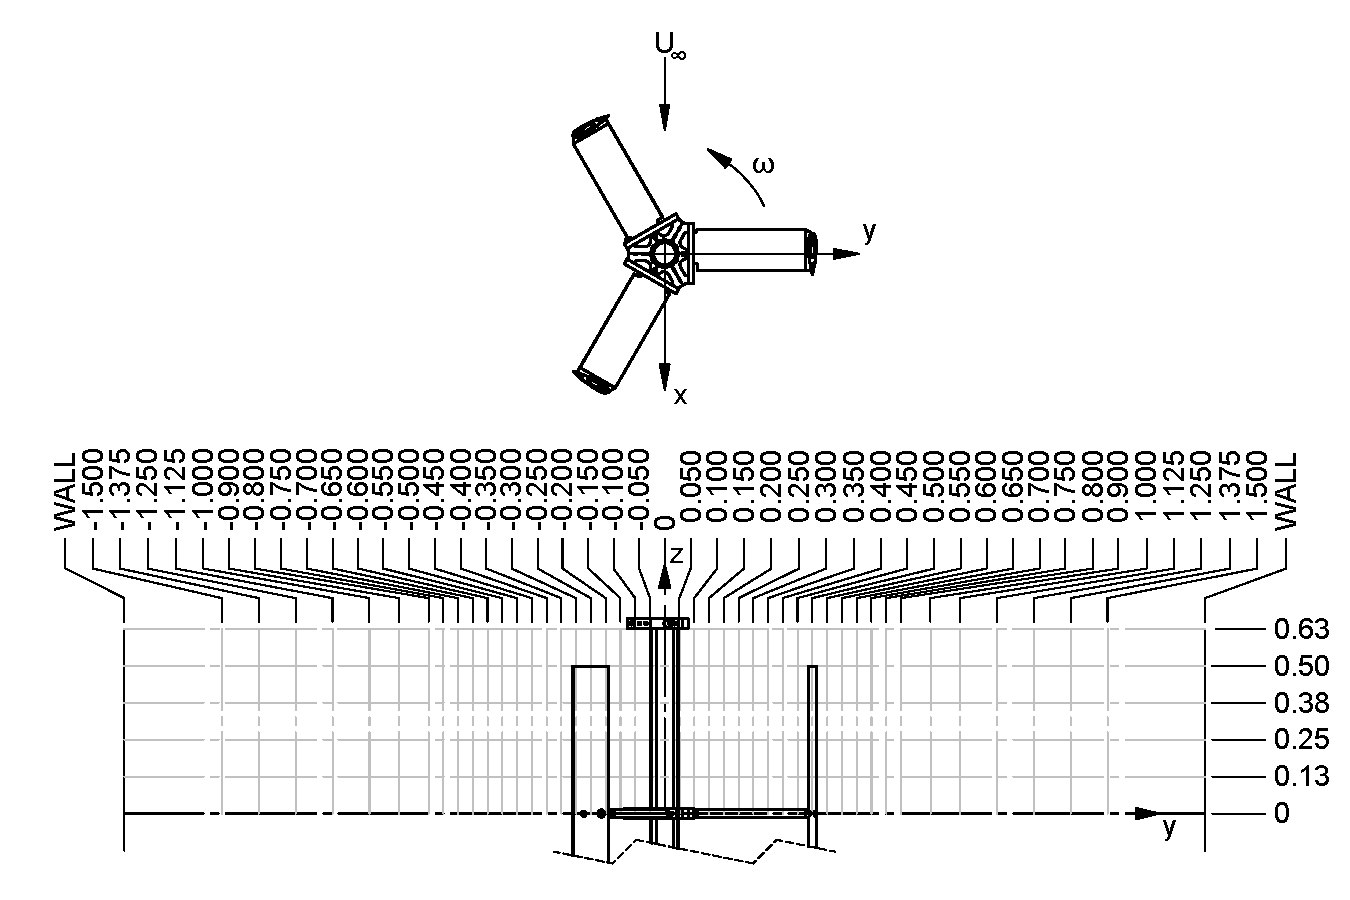
\includegraphics[width=0.9\textwidth]{figures/turbine_coordinate_system}
\caption{Wake measurement coordinate system and locations. Dimensions are in
meters.} 
\label{fig:wake_locations}
\end{figure}

\subsection{Data Processing}

From each set of tows, a standard time interval was set, and each run was
analyzed to compute statistics over this interval, truncating the end slightly
to achieve and integer number of blade passages.

\todo[inline]{Put up reduced data and processing code on figshare.}


\section{Results and Discussion}


\subsection{Performance Curves}

\todo[inline]{Put the performance curves here.}

\todo[inline]{Put asymptotic behavior here.}

\subsection{Wake Characteristics}

\todo[inline]{Put wake characteristics here. Maybe create difference plots to
show absolute differences, or RMS, or something}


\todo[inline]{Plot asymptotic behavior for a bunch of locations all on the same
plot.}


\subsubsection{Mean Kinetic Energy Transport}

The relative importance of various physical processes on mean kinetic energy
transport/recovery in the streamwise direction $\p K / \p x$ are plotted in...

\todo[inline]{Recreate the kinetic energy bar graph for all $Re$.}


\section{Conclusions}

In this study we determined that, as previously shown, turbine performance
becomes essentially $Re$-independent at a turbine diameter Reynolds number $Re_D
\approx 10^6$, or an approximate blade chord Reynolds number $Re_c \approx 2
\times 10^5$.


\acknowledgements{Acknowledgements}

The authors would like to acknowledge funding through a National Science
Foundation CAREER award (PI Wosnik, NSF-CBET 1150797, program manager Dr. Ram
Gupta), a grant through the Leslie S. Hubbard Marine Program Endowment to
purchase acoustic flow measurement instrumentation, and a grant for laboratory
infrastructure upgrades through the US Department of Energy.

\conflictofinterests{Conflicts of Interest}

The authors declare no conflict of interest.


\bibliography{../../../Library/Library}
\bibliographystyle{mdpi}

\end{document}

